\documentclass[technote,a4paper,leqno]{IEEEtran}
\pdfoutput=1

\usepackage[utf8]{inputenc} % this is needed for umlauts
\usepackage[USenglish]{babel} % this is needed for umlauts
\usepackage[T1]{fontenc}    % this is needed for correct output of umlauts in pdf
\usepackage{amsmath,amssymb}
\usepackage[absolute,overlay]{textpos}
\usepackage{tikz}
\usepackage{csquotes}
\usepackage[binary-units=true,detect-weight=true, detect-family=true]{siunitx}
\DeclareSIUnit\pixel{px}
\usepackage{caption}  % nicer captions

\usepackage{url}
\usepackage{breakurl}
\usepackage[raiselinks=true,
            bookmarks=true,
            bookmarksopenlevel=1,
            bookmarksopen=true,
            bookmarksnumbered=true,
            breaklinks,
            hyperindex=true,
            plainpages=false,
            pdfpagelabels=true,
            pdfborder={0 0 0.5}]{hyperref}
\def\UrlBreaks{\do\/\do-}

\usepackage{xspace}
\newcommand*\elide{\textup{[\,\dots]}\xspace}

\usepackage[nameinlink, noabbrev,capitalise]{cleveref}

\title{The HASYv2 dataset}
\author{%
    \IEEEauthorblockN{Martin Thoma}\\
    \IEEEauthorblockA{E-Mail: info@martin-thoma.de} % ORCID: http://orcid.org/0000-0002-6517-1690
}

\hypersetup{
    pdfauthor   = {Martin Thoma},
    pdfkeywords = {dataset},
    pdfsubject  = {HASY, HASYv2, dataset},
    pdftitle    = {The HASYv2 dataset},
}
\usepackage[inline]{enumitem}
\usepackage{longtable}
\usepackage{booktabs}       % \toprule
\usepackage{braket}         % needed for \Set
\usepackage{algorithm,algpseudocode}

% Packages for symbols
\usepackage{mathtools}
\usepackage{mathrsfs}
\def\wasyfamily{\fontencoding{U}\fontfamily{wasy}\selectfont}
\usepackage{upgreek}
\usepackage{marvosym}
\usepackage{textcomp}
\usepackage{dsfont}
\usepackage{esint}
\usepackage{cmll}
\usepackage{stmaryrd}
\usepackage{skull}

% Make document nicer
\usepackage{parskip}
\usepackage{multirow}
\usepackage{microtype}

% Variables
\newcommand{\dbTotalClasses}{369}
\newcommand{\dbTotalInstances}{\num{168233}}
\newcommand{\dbName}{HASY}
\newcommand{\dbNameVersion}{HASYv2}
\newcommand{\dbSizeMB}{34.6}
\newcommand{\dbDownloadURL}{\url{https://doi.org/10.5281/zenodo.259444}}
\newcommand{\dbMDfivesum}{fddf23f36e24b5236f6b3a0880c778e3}

% Start
\begin{document}
\maketitle
In dieser Arbeit wird der DYCOS-Algorithmus, wie er in \cite{aggarwal2011}
vorgestellt wurde, erklärt. Er arbeitet auf Graphen, deren Knoten teilweise mit
Beschriftungen versehen sind und ergänzt automatisch Beschriftungen für Knoten,
die bisher noch keine Beschriftung haben. Dieser Vorgang wird
\enquote{Klassifizierung} genannt. Dazu verwendet er die Struktur des Graphen
sowie textuelle Informationen, die den Knoten zugeordnet sind. Die in
\cite{aggarwal2011} beschriebene experimentelle Analyse ergab, dass er auch auf
dynamischen Graphen mit 19\,396 bzw. 806\,635 Knoten, von denen nur
14\,814 bzw. 18\,999 beschriftet waren, innerhalb von weniger als
einer Minute auf einem Kern einer Intel Xeon 2.5\,GHz~CPU mit 32\,G~RAM
ausgeführt werden kann.\\
Zusätzlich wird \cite{aggarwal2011} kritisch Erörtert und und es werden
mögliche Erweiterungen des DYCOS-Algorithmus vorgeschlagen.

\textbf{Keywords:} DYCOS, Label Propagation, Knotenklassifizierung

%!TEX root = main.tex
\section{Introduction}
Artificial neural networks have dozends of hyperparameters which influence
their behaviour during training and evaluation time. One parameter is the
choice of activation functions. While in principle every neuron could have a
different activation function, in practice networks only use two activation
functions: The softmax function for the output layer in order to obtain a
probability distribution over the possible classes and one activation function
for all other neurons.

Activation functions should have the following properties:
\begin{itemize}
    \item \textbf{Non-linearity}: A linear activation function in a simple feed
          forward network leads to a linear function. This means no matter how
          many layers the network uses, there is an equivalent network with
          only the input and the output layer. Please note that \glspl{CNN} are
          different. Padding and pooling are also non-linear operations.
    \item \textbf{Differentiability}: Activation functions need to be
          differentiable in order to be able to apply gradient descent. It is
          not necessary that they are differentiable at any point. In practice,
          the gradient at non-differentiable points can simply be set to zero
          in order to prevent weight updates at this point.
    \item \textbf{Non-zero gradient}: The sign function is not suitable for
          gradient descent based optimizers as its gradient is zero at all
          differentiable points. An activation function should have infinitely
          many points with non-zero gradient.
\end{itemize}

One of the simplest and most widely used activation functions for \glspl{CNN}
is \gls{ReLU}~\cite{AlexNet-2012}, but others such as
\gls{ELU}~\cite{clevert2015fast}, \gls{PReLU}~\cite{he2015delving}, softplus~\cite{7280459}
and softsign~\cite{bergstra2009quadratic} have been proposed.

Activation functions differ in the range of values and the derivative. The
definitions and other comparisons of eleven activation functions are given
in~\cref{table:activation-functions-overview}.


\section{Important Differences of Proposed Activation Functions}
Theoretical explanations why one activation function is preferable to another
in some scenarios are the following:
\begin{itemize}
    \item \textbf{Vanishing Gradient}: Activation functions like tanh and the
          logistic function saturate outside of the interval $[-5, 5]$. This
          means weight updates are very small for preceding neurons, which is
          especially a problem for very deep or recurrent networks as described
          in~\cite{bengio1994learning}. Even if the neurons learn eventually,
          learning is slower~\cite{AlexNet-2012}.
    \item \textbf{Dying ReLU}: The dying \gls{ReLU} problem is similar to the
          vanishing gradient problem. The gradient of the \gls{ReLU} function
          is~0 for all non-positive values. This means if all elements of the
          training set lead to a negative input for one neuron at any point in
          the training process, this neuron does not get any update and hence
          does not participate in the training process. This problem is
          addressed in~\cite{maas2013rectifier}.
    \item \textbf{Mean unit activation}: Some publications
          like~\cite{clevert2015fast,BatchNormalization-2015} claim that mean
          unit activations close to 0 are desirable. They claim that this
          speeds up learning by reducing the bias shift effect. The speedup
          of learning is supported by many experiments. Hence the possibility
          of negative activations is desirable.
\end{itemize}

Those considerations are listed
in~\cref{table:properties-of-activation-functions} for 11~activation functions.
Besides the theoretical properties, empiric results are provided
in~\cref{table:CIFAR-100-accuracies-activation-functions,table:CIFAR-100-timing-activation-functions}.
The baseline network was adjusted so that every activation function except the
one of the output layer was replaced by one of the 11~activation functions.

As expected, \gls{PReLU} and \gls{ELU} performed best. Unexpected was that the
logistic function, tanh and softplus performed worse than the identity and it
is unclear why the pure-softmax network performed so much better than the
logistic function.
One hypothesis why the logistic function performs so bad is that it cannot
produce negative outputs. Hence the logistic$^-$ function was developed:
\[\text{logistic}^{-}(x) = \frac{1}{1+ e^{-x}} - 0.5\]
The logistic$^-$ function has the same derivative as the logistic function and
hence still suffers from the vanishing gradient problem.
The network with the logistic$^-$ function achieves an accuracy which is
\SI{11.30}{\percent} better than the network with the logistic function, but is
still \SI{5.54}{\percent} worse than the \gls{ELU}.

Similarly, \gls{ReLU} was adjusted to have a negative output:
\[\text{ReLU}^{-}(x) = \max(-1, x) = \text{ReLU}(x+1) - 1\]
The results of \gls{ReLU}$^-$ are much worse on the training set, but perform
similar on the test set. The result indicates that the possibility of hard zero
and thus a sparse representation is either not important or similar important as
the possibility to produce negative outputs. This
contradicts~\cite{glorot2011deep,srivastava2014understanding}.

A key difference between the logistic$^-$ function and \gls{ELU} is that
\gls{ELU} does neither suffers from the vanishing gradient problem nor is its
range of values bound. For this reason, the S2ReLU activation function, defined
as
\begin{align*}
  \StwoReLU(x) &= \ReLU \left (\frac{x}{2} + 1 \right ) - \ReLU \left (-\frac{x}{2} + 1 \right)\\
  &=
  \begin{cases}-\frac{x}{2} + 1 &\text{if } x \le -2\\
               x &\text{if } -2\le x \le 2\\
               \frac{x}{2} + 1&\text{if } x > -2\end{cases}
\end{align*}
This function is similar to SReLUs as introduced in~\cite{jin2016deep}. The
difference is that S2ReLU does not introduce learnable parameters. The S2ReLU
was designed to be symmetric, be the identity close to zero and have a smaller
absolute value than the identity farther away. It is easy to compute and easy to
implement.

Those results --- not only the absolute values, but also the relative
comparison --- might depend on the network architecture, the training
algorithm, the initialization and the dataset. Results for MNIST can be found
in~\cref{table:MNIST-accuracies-activation-functions} and for HASYv2
in~\cref{table:HASYv2-accuracies-activation-functions}. For both datasets, the
logistic function has a much shorter training time and a noticeably lower test
accuracy.

\glsunset{LReLU}
\begin{table}[H]
    \centering
    \begin{tabular}{lccc}
    \toprule
    \multirow{2}{*}{Function} & Vanishing  & Negative Activation & Bound \\
                  & Gradient       & possible & activation \\\midrule
    Identity      & \cellcolor{green!25}No    & \cellcolor{green!25}  Yes    & \cellcolor{green!25}No  \\
    Logistic      & \cellcolor{red!25} Yes    & \cellcolor{red!25}   No      & \cellcolor{red!25}  Yes \\
    Logistic$^-$  & \cellcolor{red!25} Yes    & \cellcolor{green!25}  Yes    & \cellcolor{red!25}  Yes \\
    Softmax        & \cellcolor{red!25} Yes    & \cellcolor{green!25}  Yes    & \cellcolor{red!25}  Yes \\
    tanh          & \cellcolor{red!25} Yes    & \cellcolor{green!25}  Yes    & \cellcolor{red!25}  Yes \\
    Softsign      & \cellcolor{red!25} Yes    & \cellcolor{green!25}Yes      & \cellcolor{red!25}   Yes \\
    ReLU          & \cellcolor{yellow!25}Yes\footnotemark & \cellcolor{red!25} No & \cellcolor{yellow!25}Half-sided \\
    Softplus      & \cellcolor{green!25}No    & \cellcolor{red!25}   No      & \cellcolor{yellow!25}Half-sided \\
    S2ReLU        & \cellcolor{green!25}No    & \cellcolor{green!25}Yes      & \cellcolor{green!25} No \\
    \gls{LReLU}/PReLU   & \cellcolor{green!25}No    & \cellcolor{green!25}Yes      & \cellcolor{green!25} No \\
    ELU           & \cellcolor{green!25}No    & \cellcolor{green!25}Yes      & \cellcolor{green!25} No \\
    \bottomrule
    \end{tabular}
    \caption[Activation function properties]{Properties of activation functions.}
    \label{table:properties-of-activation-functions}
\end{table}
\footnotetext{The dying ReLU problem is similar to the vanishing gradient problem.}

\begin{table}[H]
    \centering
    \begin{tabular}{lccclllll}
    \toprule
    \multirow{2}{*}{Function} & \multicolumn{2}{c}{Inference per}                                & Training                            & \multirow{2}{*}{Epochs} & Mean total        \\\cline{2-3}
                              & 1 Image                        & 128                             & time                                &                         & training time     \\\midrule
    Identity                  & \SI{8}{\milli\second}          & \SI{42}{\milli\second}          & \SI{31}{\second\per\epoch}          & 108 -- \textbf{148}     &\SI{3629}{\second} \\
    Logistic                  & \SI{6}{\milli\second}          & \textbf{\SI{31}{\milli\second}} & \SI{24}{\second\per\epoch}          & \textbf{101} -- 167     &\textbf{\SI{2234}{\second}} \\
    Logistic$^-$              & \SI{6}{\milli\second}          & \textbf{\SI{31}{\milli\second}} & \textbf{\SI{22}{\second\per\epoch}} & 133 -- 255              &\SI{3421}{\second} \\
    Softmax                   & \SI{7}{\milli\second}          & \SI{37}{\milli\second}          & \SI{33}{\second\per\epoch}          & 127 -- 248              &\SI{5250}{\second} \\
    Tanh                      & \SI{6}{\milli\second}          & \textbf{\SI{31}{\milli\second}} & \SI{23}{\second\per\epoch}          & 125 -- 211              &\SI{3141}{\second} \\
    Softsign                  & \SI{6}{\milli\second}          & \textbf{\SI{31}{\milli\second}} & \SI{23}{\second\per\epoch}          & 122 -- 205              &\SI{3505}{\second} \\
    \gls{ReLU}                & \SI{6}{\milli\second}          & \textbf{\SI{31}{\milli\second}} & \SI{23}{\second\per\epoch}          & 118 -- 192              &\SI{3449}{\second} \\
    Softplus                  & \SI{6}{\milli\second}          & \textbf{\SI{31}{\milli\second}} & \SI{24}{\second\per\epoch}          & \textbf{101} -- 165     &\SI{2718}{\second} \\
    S2ReLU                    & \textbf{\SI{5}{\milli\second}} & \SI{32}{\milli\second}          & \SI{26}{\second\per\epoch}          & 108 -- 209              &\SI{3231}{\second} \\
    \gls{LReLU}               & \SI{7}{\milli\second}          & \SI{34}{\milli\second}          & \SI{25}{\second\per\epoch}          & 109 -- 198              &\SI{3388}{\second} \\
    \gls{PReLU}               & \SI{7}{\milli\second}          & \SI{34}{\milli\second}          & \SI{28}{\second\per\epoch}          & 131 -- 215              &\SI{3970}{\second} \\
    \gls{ELU}                 & \SI{6}{\milli\second}          & \textbf{\SI{31}{\milli\second}} & \SI{23}{\second\per\epoch}          & 146 -- 232              &\SI{3692}{\second} \\
    \bottomrule
    \end{tabular}
    \caption[Activation function timing results on CIFAR-100]{Training time and
             inference time of adjusted baseline models trained with different
             activation functions on GTX~970 \glspl{GPU} on CIFAR-100. It was
             expected that the identity is the fastest function. This result is
             likely an implementation specific problem of Keras~2.0.4 or
             Tensorflow~1.1.0.}
    \label{table:CIFAR-100-timing-activation-functions}
\end{table}

\begin{table}[H]
    \centering
    \begin{tabular}{lccccc}
    \toprule
    \multirow{2}{*}{Function} & \multicolumn{2}{c}{Single model}              & Ensemble & \multicolumn{2}{c}{Epochs}\\\cline{2-3}\cline{5-6}
                              & Accuracy             & std                    & Accuracy & Range & Mean \\\midrule
    Identity                  & \SI{99.45}{\percent} & $\sigma=0.09$          & \SI{99.63}{\percent} & 55 -- \hphantom{0}77  & 62.2\\%TODO: Really?
    Logistic                  & \SI{97.27}{\percent} & $\sigma=2.10$          & \SI{99.48}{\percent} & \textbf{37} -- \hphantom{0}76  & \textbf{54.5}\\
    Softmax                   & \SI{99.60}{\percent} & $\boldsymbol{\sigma=0.03}$& \SI{99.63}{\percent} & 44 -- \hphantom{0}73  & 55.6\\
    Tanh                      & \SI{99.40}{\percent} & $\sigma=0.09$          & \SI{99.57}{\percent} & 56 -- \hphantom{0}80  & 67.6\\
    Softsign                  & \SI{99.40}{\percent} & $\sigma=0.08$          & \SI{99.57}{\percent} & 72 -- 101             & 84.0\\
    \gls{ReLU}                & \textbf{\SI{99.62}{\percent}} & \textbf{$\sigma=0.04$} & \textbf{\SI{99.73}{\percent}} & 51 -- \hphantom{0}94 & 71.7\\
    Softplus                  & \SI{99.52}{\percent} & $\sigma=0.05$          & \SI{99.62}{\percent} & 62 -- \hphantom{0}\textbf{70}  & 68.9\\
    \gls{PReLU}               & \SI{99.57}{\percent} & $\sigma=0.07$          & \textbf{\SI{99.73}{\percent}} & 44 -- \hphantom{0}89 & 71.2\\
    \gls{ELU}                 & \SI{99.53}{\percent} & $\sigma=0.06$          & \SI{99.58}{\percent} & 45 -- 111 & 72.5\\
    \bottomrule
    \end{tabular}
    \caption[Activation function evaluation results on MNIST]{Test accuracy of
             adjusted baseline models trained with different activation
             functions on MNIST.}
    \label{table:MNIST-accuracies-activation-functions}
\end{table}
\glsreset{LReLU}


\bibliographystyle{IEEEtranSA}
\bibliography{literatur}
%!TEX root = main.tex

\appendix
\section*{Obtaining the data}
The data can be found at \dbDownloadURL. It is a \verb+tar.gz+ file of
\SI{\dbSizeMB}{\mega\byte}. The file can be verified with the MD5sum

\texttt{\dbMDfivesum}

The data is published under the ODbL~license. If you use
the \dbName~dataset, please cite this paper.

The \verb+tar.gz+ archive contains all data as png images and CSV files with
labels. The CSV files have the
columns \verb+path,symbol_id,latex,user_id+ with a header row. The \verb+path+ is the
relative path to a training example to the CSV file, e.g. \verb+../hasy-data/v2-00000.png+. The
\verb+symbol_id+ is an internal numeric identifier for the symbol class. The
website \href{http://write-math.com/symbol/?id=968}{write-math.com/symbol/?id=[symbol\_id]}
gives information related to the symbol. The column \verb+latex+ contains the
\LaTeX{} command associated with the class.
\onecolumn
%!TEX root = "../thesis.tex"
\section*{Symbol Classes}
            \begin{longtable}{lc|lc}
                \toprule
                \LaTeX & Rendered & \LaTeX & Rendered \\
                \midrule
                \endhead
                \hline \multicolumn{4}{r}{{Continued on next page}} \\
                \endfoot
                \bottomrule
                \caption{112 symbols of \dbName.}
                \endlastfoot
\verb+\&+ & $\&$ &\verb+\nmid+ & $\nmid$\\
\verb+\Im+ & $\Im$ &\verb+\nvDash+ & $\nvDash$\\
\verb+\Re+ & $\Re$ &\verb+\int+ & $\int$\\
\verb+\S+ & $\S$ &\verb+\fint+ & $\fint$\\
\verb+\Vdash+ & $\Vdash$ &\verb+\odot+ & $\odot$\\
\verb+\aleph+ & $\aleph$ &\verb+\oiint+ & $\oiint$\\
\verb+\amalg+ & $\amalg$ &\verb+\oint+ & $\oint$\\
\verb+\angle+ & $\angle$ &\verb+\varoiint+ & $\varoiint$\\
\verb+\ast+ & $\ast$ &\verb+\ominus+ & $\ominus$\\
\verb+\asymp+ & $\asymp$ &\verb+\oplus+ & $\oplus$\\
\verb+\backslash+ & $\backslash$ &\verb+\otimes+ & $\otimes$\\
\verb+\between+ & $\between$ &\verb+\parallel+ & $\parallel$\\
\verb+\blacksquare+ & $\blacksquare$ &\verb+\parr+ & $\parr$\\
\verb+\blacktriangleright+ & $\blacktriangleright$ &\verb+\partial+ & $\partial$\\
\verb+\bot+ & $\bot$ &\verb+\perp+ & $\perp$\\
\verb+\bowtie+ & $\bowtie$ &\verb+\pitchfork+ & $\pitchfork$\\
\verb+\boxdot+ & $\boxdot$ &\verb+\pm+ & $\pm$\\
\verb+\boxplus+ & $\boxplus$ &\verb+\prime+ & $\prime$\\
\verb+\boxtimes+ & $\boxtimes$ &\verb+\prod+ & $\prod$\\
\verb+\bullet+ & $\bullet$ &\verb+\propto+ & $\propto$\\
\verb+\checkmark+ & $\checkmark$ &\verb+\rangle+ & $\rangle$\\
\verb+\circ+ & $\circ$ &\verb+\rceil+ & $\rceil$\\
\verb+\circledR+ & $\circledR$ &\verb+\rfloor+ & $\rfloor$\\
\verb+\circledast+ & $\circledast$ &\verb+\rrbracket+ & $\rrbracket$\\
\verb+\circledcirc+ & $\circledcirc$ &\verb+\rtimes+ & $\rtimes$\\
\verb+\clubsuit+ & $\clubsuit$ &\verb+\sharp+ & $\sharp$\\
\verb+\coprod+ & $\coprod$ &\verb+\sphericalangle+ & $\sphericalangle$\\
\verb+\copyright+ & $\copyright$ &\verb+\sqcap+ & $\sqcap$\\
\verb+\dag+ & $\dag$ &\verb+\sqcup+ & $\sqcup$\\
\verb+\dashv+ & $\dashv$ &\verb+\sqrt{}+ & $\sqrt{}$\\
\verb+\diamond+ & $\diamond$ &\verb+\square+ & $\square$\\
\verb+\diamondsuit+ & $\diamondsuit$ &\verb+\star+ & $\star$\\
\verb+\div+ & $\div$ &\verb+\sum+ & $\sum$\\
\verb+\ell+ & $\ell$ &\verb+\times+ & $\times$\\
\verb+\flat+ & $\flat$ &\verb+\top+ & $\top$\\
\verb+\frown+ & $\frown$ &\verb+\triangle+ & $\triangle$\\
\verb+\guillemotleft+ & $\guillemotleft$ &\verb+\triangledown+ & $\triangledown$\\
\verb+\hbar+ & $\hbar$ &\verb+\triangleleft+ & $\triangleleft$\\
\verb+\heartsuit+ & $\heartsuit$ &\verb+\trianglelefteq+ & $\trianglelefteq$\\
\verb+\infty+ & $\infty$ &\verb+\triangleq+ & $\triangleq$\\
\verb+\langle+ & $\langle$ &\verb+\triangleright+ & $\triangleright$\\
\verb+\lceil+ & $\lceil$ &\verb+\uplus+ & $\uplus$\\
\verb+\lfloor+ & $\lfloor$ &\verb+\vDash+ & $\vDash$\\
\verb+\lhd+ & $\lhd$ &\verb+\varnothing+ & $\varnothing$\\
\verb+\lightning+ & $\lightning$ &\verb+\varpropto+ & $\varpropto$\\
\verb+\llbracket+ & $\llbracket$ &\verb+\vartriangle+ & $\vartriangle$\\
\verb+\lozenge+ & $\lozenge$ &\verb+\vdash+ & $\vdash$\\
\verb+\ltimes+ & $\ltimes$ &\verb+\with+ & $\with$\\
\verb+\mathds{1}+ & $\mathds{1}$ &\verb+\wp+ & $\wp$\\
\verb+\mathsection+ & $\mathsection$ &\verb+\wr+ & $\wr$\\
\verb+\mid+ & $\mid$ &\verb+\{+ & $\{$\\
\verb+\models+ & $\models$ &\verb+\|+ & $\|$\\
\verb+\mp+ & $\mp$ &\verb+\}+ & $\}$\\
\verb+\multimap+ & $\multimap$ &\verb+\vee+ & $\vee$\\
\verb+\nabla+ & $\nabla$ &\verb+\wedge+ & $\wedge$\\
\verb+\neg+ & $\neg$ &\verb+\barwedge+ & $\barwedge$
    \label{table:symbols-of-db-0}
    \end{longtable}


\begin{table}[ht]
        \centering

            \begin{tabular}{lc|lc|lc|lc}
                \toprule
                \LaTeX & Rendered & \LaTeX & Rendered & \LaTeX & Rendered & \LaTeX & Rendered \\
                \midrule
\verb+\#+ & $\#$ &\verb+A+ & $A$ &\verb+S+ & $S$ &\verb+i+ & $i$\\
\verb+\$+ & $\$$ &\verb+B+ & $B$ &\verb+T+ & $T$ &\verb+j+ & $j$\\
\verb+\%+ & $\%$ &\verb+C+ & $C$ &\verb+U+ & $U$ &\verb+k+ & $k$\\
\verb+++ & $+$ &\verb+D+ & $D$ &\verb+V+ & $V$ &\verb+l+ & $l$\\
\verb+-+ & $-$ &\verb+E+ & $E$ &\verb+W+ & $W$ &\verb+m+ & $m$\\
\verb+/+ & $/$ &\verb+F+ & $F$ &\verb+X+ & $X$ &\verb+n+ & $n$\\
\verb+0+ & $0$ &\verb+G+ & $G$ &\verb+Y+ & $Y$ &\verb+o+ & $o$\\
\verb+1+ & $1$ &\verb+H+ & $H$ &\verb+Z+ & $Z$ &\verb+p+ & $p$\\
\verb+2+ & $2$ &\verb+I+ & $I$ &\verb+[+ & $[$ &\verb+q+ & $q$\\
\verb+3+ & $3$ &\verb+J+ & $J$ &\verb+]+ & $]$ &\verb+r+ & $r$\\
\verb+4+ & $4$ &\verb+K+ & $K$ &\verb+a+ & $a$ &\verb+s+ & $s$\\
\verb+5+ & $5$ &\verb+L+ & $L$ &\verb+b+ & $b$ &\verb+u+ & $u$\\
\verb+6+ & $6$ &\verb+M+ & $M$ &\verb+c+ & $c$ &\verb+v+ & $v$\\
\verb+7+ & $7$ &\verb+N+ & $N$ &\verb+d+ & $d$ &\verb+w+ & $w$\\
\verb+8+ & $8$ &\verb+O+ & $O$ &\verb+e+ & $e$ &\verb+x+ & $x$\\
\verb+9+ & $9$ &\verb+P+ & $P$ &\verb+f+ & $f$ &\verb+y+ & $y$\\
\verb+<+ & $<$ &\verb+Q+ & $Q$ &\verb+g+ & $g$ &\verb+z+ & $z$\\
\verb+>+ & $>$ &\verb+R+ & $R$ &\verb+h+ & $h$ &\verb+|+ & $|$\\

        \bottomrule
    \end{tabular}

    \caption{72 ASCII symbols of \dbName, including all
             ten digits, the Latin alphabet in lower and upper case and
             a few more symbols.}
    \label{table:symbols-of-db-1}
\end{table}


\begin{table}[ht]
        \centering
            \begin{tabular}{lc|lc|lc}
                \toprule
                \LaTeX & Rendered & \LaTeX & Rendered & \LaTeX & Rendered \\
                \midrule
\verb+\approx+ & $\approx$ &\verb+\geqslant+ & $\geqslant$ &\verb+\lesssim+ & $\lesssim$\\
\verb+\doteq+ & $\doteq$ &\verb+\neq+ & $\neq$ &\verb+\backsim+ & $\backsim$\\
\verb+\simeq+ & $\simeq$ &\verb+\not\equiv+ & $\not\equiv$ &\verb+\sim+ & $\sim$\\
\verb+\equiv+ & $\equiv$ &\verb+\preccurlyeq+ & $\preccurlyeq$ &\verb+\succ+ & $\succ$\\
\verb+\geq+ & $\geq$ &\verb+\preceq+ & $\preceq$ &\verb+\prec+ & $\prec$\\
\verb+\leq+ & $\leq$ &\verb+\succeq+ & $\succeq$ &\verb+\gtrless+ & $\gtrless$\\
\verb+\leqslant+ & $\leqslant$ &\verb+\gtrsim+ & $\gtrsim$ &\verb+\cong+ & $\cong$\\
        \bottomrule
    \end{tabular}

    \caption{21 symbols which are in \dbName and indicate a relationship.}
    \label{table:symbols-of-db-2}
\end{table}


\begin{table}[ht]
        \centering

            \begin{tabular}{lc|lc}
                \toprule
                \LaTeX & Rendered & \LaTeX & Rendered \\
                \midrule
\verb+\Downarrow+ & $\Downarrow$ &\verb+\nrightarrow+ & $\nrightarrow$\\
\verb+\Leftarrow+ & $\Leftarrow$ &\verb+\rightarrow+ & $\rightarrow$\\
\verb+\Leftrightarrow+ & $\Leftrightarrow$ &\verb+\rightleftarrows+ & $\rightleftarrows$\\
\verb+\Longleftrightarrow+ & $\Longleftrightarrow$ &\verb+\rightrightarrows+ & $\rightrightarrows$\\
\verb+\Longrightarrow+ & $\Longrightarrow$ &\verb+\rightsquigarrow+ & $\rightsquigarrow$\\
\verb+\Rightarrow+ & $\Rightarrow$ &\verb+\searrow+ & $\searrow$\\
\verb+\circlearrowleft+ & $\circlearrowleft$ &\verb+\shortrightarrow+ & $\shortrightarrow$\\
\verb+\circlearrowright+ & $\circlearrowright$ &\verb+\twoheadrightarrow+ & $\twoheadrightarrow$\\
\verb+\curvearrowright+ & $\curvearrowright$ &\verb+\uparrow+ & $\uparrow$\\
\verb+\downarrow+ & $\downarrow$ &\verb+\rightharpoonup+ & $\rightharpoonup$\\
\verb+\hookrightarrow+ & $\hookrightarrow$ &\verb+\rightleftharpoons+ & $\rightleftharpoons$\\
\verb+\leftarrow+ & $\leftarrow$ &\verb+\longmapsto+ & $\longmapsto$\\
\verb+\leftrightarrow+ & $\leftrightarrow$ &\verb+\mapsfrom+ & $\mapsfrom$\\
\verb+\longrightarrow+ & $\longrightarrow$ &\verb+\mapsto+ & $\mapsto$\\
\verb+\nRightarrow+ & $\nRightarrow$ &\verb+\leadsto+ & $\leadsto$\\
\verb+\nearrow+ & $\nearrow$ &\verb+\upharpoonright+ & $\upharpoonright$\\

        \bottomrule
    \end{tabular}

    \caption{32 arrow symbols of \dbName.}
    \label{table:symbols-of-db-3}
\end{table}


\begin{table}[ht]
        \centering

            \begin{tabular}{lc|lc|lc}
                \toprule
                \LaTeX & Rendered & \LaTeX & Rendered & \LaTeX & Rendered \\
                \midrule
\verb+\alpha+ & $\alpha$ &\verb+\xi+ & $\xi$ &\verb+\Xi+ & $\Xi$\\
\verb+\beta+ & $\beta$ &\verb+\pi+ & $\pi$ &\verb+\Pi+ & $\Pi$\\
\verb+\gamma+ & $\gamma$ &\verb+\rho+ & $\rho$ &\verb+\Sigma+ & $\Sigma$\\
\verb+\delta+ & $\delta$ &\verb+\sigma+ & $\sigma$ &\verb+\Phi+ & $\Phi$\\
\verb+\epsilon+ & $\epsilon$ &\verb+\tau+ & $\tau$ &\verb+\Psi+ & $\Psi$\\
\verb+\zeta+ & $\zeta$ &\verb+\phi+ & $\phi$ &\verb+\Omega+ & $\Omega$\\
\verb+\eta+ & $\eta$ &\verb+\chi+ & $\chi$ &\verb+\varepsilon+ & $\varepsilon$\\
\verb+\theta+ & $\theta$ &\verb+\psi+ & $\psi$ &\verb+\varkappa+ & $\varkappa$\\
\verb+\iota+ & $\iota$ &\verb+\omega+ & $\omega$ &\verb+\varpi+ & $\varpi$\\
\verb+\kappa+ & $\kappa$ &\verb+\Gamma+ & $\Gamma$ &\verb+\varrho+ & $\varrho$\\
\verb+\lambda+ & $\lambda$ &\verb+\Delta+ & $\Delta$ &\verb+\varphi+ & $\varphi$\\
\verb+\mu+ & $\mu$ &\verb+\Theta+ & $\Theta$ &\verb+\vartheta+ & $\vartheta$\\
\verb+\nu+ & $\nu$ &\verb+\Lambda+ & $\Lambda$ &\verb+ + & $ $\\

        \bottomrule
    \end{tabular}

    \caption{All Greek letters and some variations of Greek letters were
             used for evaluation. 38 of them are in this table, the rest
             is identical to Latin letters.}
    \label{table:symbols-of-db-4}
\end{table}


\begin{table}[ht]
        \centering

            \begin{tabular}{lc|lc|lc}
                \toprule
                \LaTeX & Rendered & \LaTeX & Rendered & \LaTeX & Rendered \\
                \midrule
\verb+\mathcal{A}+ & $\mathcal{A}$ &\verb+\mathcal{T}+ & $\mathcal{T}$ &\verb+\mathds{Z}+ & $\mathds{Z}$\\
\verb+\mathcal{B}+ & $\mathcal{B}$ &\verb+\mathcal{U}+ & $\mathcal{U}$ &\verb+\mathfrak{A}+ & $\mathfrak{A}$\\
\verb+\mathcal{C}+ & $\mathcal{C}$ &\verb+\mathcal{X}+ & $\mathcal{X}$ &\verb+\mathfrak{M}+ & $\mathfrak{M}$\\
\verb+\mathcal{D}+ & $\mathcal{D}$ &\verb+\mathcal{Z}+ & $\mathcal{Z}$ &\verb+\mathfrak{S}+ & $\mathfrak{S}$\\
\verb+\mathcal{E}+ & $\mathcal{E}$ &\verb+\mathbb{H}+ & $\mathbb{H}$ &\verb+\mathfrak{X}+ & $\mathfrak{X}$\\
\verb+\mathcal{F}+ & $\mathcal{F}$ &\verb+\mathbb{N}+ & $\mathbb{N}$ &\verb+\mathscr{A}+ & $\mathscr{A}$\\
\verb+\mathcal{G}+ & $\mathcal{G}$ &\verb+\mathbb{Q}+ & $\mathbb{Q}$ &\verb+\mathscr{C}+ & $\mathscr{C}$\\
\verb+\mathcal{H}+ & $\mathcal{H}$ &\verb+\mathbb{R}+ & $\mathbb{R}$ &\verb+\mathscr{D}+ & $\mathscr{D}$\\
\verb+\mathcal{L}+ & $\mathcal{L}$ &\verb+\mathbb{Z}+ & $\mathbb{Z}$ &\verb+\mathscr{E}+ & $\mathscr{E}$\\
\verb+\mathcal{M}+ & $\mathcal{M}$ &\verb+\mathds{C}+ & $\mathds{C}$ &\verb+\mathscr{F}+ & $\mathscr{F}$\\
\verb+\mathcal{N}+ & $\mathcal{N}$ &\verb+\mathds{E}+ & $\mathds{E}$ &\verb+\mathscr{H}+ & $\mathscr{H}$\\
\verb+\mathcal{O}+ & $\mathcal{O}$ &\verb+\mathds{N}+ & $\mathds{N}$ &\verb+\mathscr{L}+ & $\mathscr{L}$\\
\verb+\mathcal{P}+ & $\mathcal{P}$ &\verb+\mathds{P}+ & $\mathds{P}$ &\verb+\mathscr{P}+ & $\mathscr{P}$\\
\verb+\mathcal{R}+ & $\mathcal{R}$ &\verb+\mathds{Q}+ & $\mathds{Q}$ &\verb+\mathscr{S}+ & $\mathscr{S}$\\
\verb+\mathcal{S}+ & $\mathcal{S}$ &\verb+\mathds{R}+ & $\mathds{R}$ &\verb+ + & $ $\\

        \bottomrule
    \end{tabular}

    \caption{44 variants of Latin letters in \dbName.}
    \label{table:symbols-of-db-5}
\end{table}


\begin{table}[ht]
        \centering

            \begin{tabular}{lc|lc|lc}
                \toprule
                \LaTeX & Rendered & \LaTeX & Rendered & \LaTeX & Rendered \\
                \midrule
\verb+\therefore+ & $\therefore$ &\verb+\cdot+  & $\cdot$  &\verb+\dots+  & $\dots$\\
\verb+\because+   & $\because$   &\verb+\vdots+ & $\vdots$ &\verb+\ddots+ & $\ddots$\\
\verb+\dotsc+     & $\dotsc$     &\verb+ +      &          &\verb+ +      &  \\
        \bottomrule
    \end{tabular}

    \caption{7 symbols that contain only dots in \dbName.}
    \label{table:symbols-of-db-6}
\end{table}


\begin{table}[ht]
        \centering
            \begin{tabular}{lc|lc|lc|lc|lc}
                \toprule
                \LaTeX & R & \LaTeX & R & \LaTeX & R &  \LaTeX & R & \LaTeX & R \\
                \midrule
\verb+\AA+ & {\r A}                                                           &\verb+\L+       & 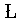
\includegraphics[height=12.3pt, keepaspectratio]{symbols/L.pdf} &\verb+\male+     & {\mbox {\wasyfamily \char 26}}                         &\verb+\ohm+      &  $\Omega $                     &\verb+\sun+       & {\mbox {\wasyfamily \char 46}} \\
\verb+\AE+ & \includegraphics[height=12.3pt, keepaspectratio]{symbols/AE.pdf} &\verb+\O+       & 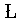
\includegraphics[height=12.3pt, keepaspectratio]{symbols/L.pdf} &\verb+\mars+     & {\leavevmode \lower 0.2ex\hbox {\wasyfamily \char 26}} &\verb+\fullmoon+ & {\mbox {\wasyfamily \char 35}} &\verb+\degree+    & {\ensuremath {^\circ }}\\
\verb+\aa+ & {\r a}                                                           &\verb+\o+       & 
\includegraphics[height=12.3pt, keepaspectratio]{symbols/o.pdf} &\verb+\female+   & {\mbox {\wasyfamily \char 25}}                         &\verb+\leftmoon+ & {\mbox {\wasyfamily \char 36}} &\verb+\iddots+    & 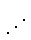
\includegraphics[height=12.3pt, keepaspectratio]{symbols/iddots.pdf}\\
\verb+\ae+ & \includegraphics[height=12.3pt, keepaspectratio]{symbols/AE.pdf} &\verb+\Bowtie+  & {\mbox {\wasyfamily \char 49}}                                  &\verb+\venus+    & {\leavevmode \raise 0.2ex\hbox {\wasyfamily \char 25}} &\verb+\checked+  & {\mbox {\wasyfamily \char 8}}  &\verb+\diameter+  & {\mbox {\wasyfamily \char 31}} \\
\verb+\ss+ & 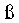
\includegraphics[height=12.3pt, keepaspectratio]{symbols/ss.pdf} &\verb+\celsius+ & $^\circ \mathrm {C}$                                            &\verb+\astrosun+ & {\mbox {$\odot $}}                                     &\verb+\pounds+   & \textsterling                  &\verb+\mathbb{1}+ & 
\includegraphics{symbols/mathbb1.pdf}\\
        \bottomrule
    \end{tabular}
    \caption{25 symbols of \dbName.}
    \label{table:symbols-of-db-7}
\end{table}


\begin{table}[ht]
        \centering

            \begin{tabular}{lc|lc|lc}
                \toprule
                \LaTeX & Rendered & \LaTeX & Rendered & \LaTeX & Rendered \\
                \midrule
\verb+\cup+ & $\cup$ &\verb+\varsubsetneq+ & $\varsubsetneq$ &\verb+\exists+ & $\exists$\\
\verb+\cap+ & $\cap$ &\verb+\nsubseteq+ & $\nsubseteq$ &\verb+\nexists+ & $\nexists$\\
\verb+\emptyset+ & $\emptyset$ &\verb+\sqsubseteq+ & $\sqsubseteq$ &\verb+\forall+ & $\forall$\\
\verb+\setminus+ & $\setminus$ &\verb+\subseteq+ & $\subseteq$ &\verb+\in+ & $\in$\\
\verb+\supset+ & $\supset$ &\verb+\subsetneq+ & $\subsetneq$ &\verb+\ni+ & $\ni$\\
\verb+\subset+ & $\subset$ &\verb+\supseteq+ & $\supseteq$ &\verb+\notin+ & $\notin$\\

        \bottomrule
    \end{tabular}

    \caption{18 set related symbols of \dbName.}
    \label{table:symbols-of-db-8}
\end{table}
\clearpage
\twocolumn


\end{document}
